\section{Resource Sharing}
\textit{Resource sharing}  is the assignment of a resource to more than one operation. The primary goal of resource sharing is to reduce the area of a circuit, by allowing multiple non-concurrent operations to share the same hardware operator. Resource sharing is often mandatory to meet specified upper bounds on the circuit area.\\
\textit{Resource  binding}  is the explicit definition of a mapping between the operations and the resources.\\
When considering \textit{resource-dominated circuits} that have been scheduled under resource constraints, the area is already determined by the resource usage. Thus binding and sharing serve just the purpose of refining the structural information so that connectivity synthesis can be performed.
\subsection{Binding/Sharing scenario}
\begin{itemize}
\item  \textbf{Dedicated resources} (min Latency, MAX Area): one resource per operation, no sharing thus Binding intrinsically defined
\item  \textbf{One multi-task resource} (Area is fixed, Latency defined by scheduling): an arithmetic co-processor that computes all necessary operations, max sharing, no binding.
\item  \textbf{One resource per type} (Area defined by sharing): there are adder, multiplier, ecc. Binding is partially defined, sharing (all operations of the same type use the same resource, the goal of the optimization problem)
\item \textbf{Many resources per type} (Area defined by binding; Sharing affected by type selection). Different types of the same operation: for the adder Ripple-carry, Carry-save, Carry-lookahead; for the multiplier Wallace, Partial Product Mult. Binding and Sharing.
\end{itemize}

\subsection{Perfect  Graphs}
Each undirected graph can be characterized by  four  numbers:
\begin{enumerate}
\item $ \omega(G) $ \textit{clique number}: the cardinality of its largest clique, called  maximum clique
\item $ K(G) $  \textit{clique cover number}: the cardinality of a minimum clique partition is equal to the cardinality of a minimum clique cover
\item $ \alpha(G) $ \textit{ stability number}: the cardinality of its largest stable set. A  stable set  is a subset of vertices with the property that no two vertices in the stable set are adjacent
\item $ \chi(G) $ \textit{chromatic number}: the cardinality of the minimum number of colors needed
to color the vertices into subsets, such that each is a stable set
\end{enumerate}
A graph is said to be  \textit{partitioned into cliques} if its vertex set is partitioned into (disjoint) subsets, each one inducing a clique. Similarly, a graph is said to be  \textit{covered} by  cliques  when the vertex set can  be  subdivided into (possibly overlapping) subsets, each one inducing a clique.\\
The size of the maximum clique is a lower bound for the chromatic number, because all vertices in that clique must be colored differently
\[ \omega(G) \leq \chi(G) \]
Similarly, the stability number is a lower bound for the clique cover number, since each vertex of the stable set must belong to a different clique of a clique cover
\[ \alpha(G) \leq K(G) \]
A graph is said to he  \textit{perfect}  when the inequalities can be replaced by equalities.
\bigskip \\
An \textit{interval graph} is a graph whose vertices can be put in one-to-one correspondence with a set of  intervals, so that two vertices are adjacent if and only if the corresponding intervals intersect.
\begin{figure}[H]
    \centering
    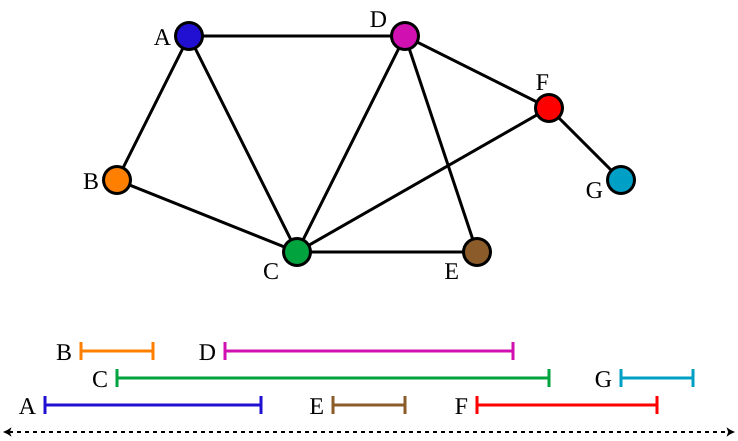
\includegraphics[width=0.45\textwidth]{./Cap5/Images/Image05.png}
    \caption{interval graph}
    \label{fig:intervalgraph}
\end{figure}
A graph  is a  \textit{comparability graph}  if it satisfies the  \textit{transitive orientation property},  i.e., if it has an orientation such that in the resulting directed graph
\[G(V,F),\:\: \lbrace (v_i,v_j)\in F\:and\: (v_j,v_k)\in F \rbrace \Rightarrow (v_i,v_k)\in F \]

\paragraph{Example}
Consider the graph of Figure \ref{fig:Undirec}a.
\begin{itemize}
\item The size of the maximum clique $ \lbrace v_1,v_2,v_3 \rbrace $ is $ \omega(G)=3 $
\item The graph can be partitioned into cliques $ \lbrace v_1,v_2,v_3 \rbrace $ and $ \lbrace v_4 \rbrace $.  Alternatively,  it  can be covered by cliques $ \lbrace v_1,v_2,v_3 \rbrace $ and $ \lbrace v_1,v_3,v_4 \rbrace $. The clique cover number $ K(G) = 2$
\item  The largest stable set is  $ \lbrace v_2,v_4 \rbrace $.  Thus, the stability number is $ \alpha(G) = 2$ 
\item  A  minimum coloring would require three colors for $ \lbrace v_1,v_2,v_3 \rbrace $. Vertex $ \lbrace v_4 \rbrace $ can have the same color as $ \lbrace v_2 \rbrace $.  Hence the chromatic number $ \chi(G)=3$.
\end{itemize}
Because $ \alpha(G) = K(G) = 2 $, the graph is perfect.\\
Figure \ref{fig:Undirec}(b) shows an orientation that does not satisfy the transitive property (because there is no edge between vertices $ v_2 $  and  $ v_4 $).  Nevertheless, the orientation shown in Figure  \ref{fig:Undirec}(c) (obtained by reversing the direction of the edge between $ v_3 $  and  $ v_4 $)  has the transitive property. Hence the graph of Figure  \ref{fig:Undirec}(a) is a comparability graph.
\begin{figure}[H]
    \centering
    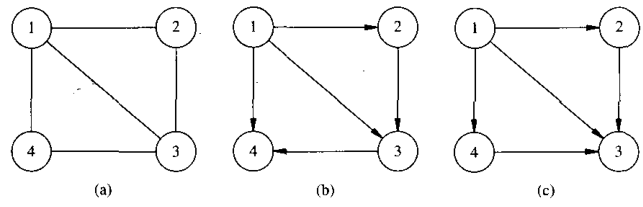
\includegraphics[width=0.45\textwidth]{./Cap5/Images/Image04.png}
    \caption{(a)  Undirected  graph.  (b)  An  orientation.  (c)  A  transitive  orienlarion.}
    \label{fig:Undirec}
\end{figure}	



\subsection{Sharing and binding for resource-dominated circuits}
We consider sharing and binding problems for resource-dominated circuits modeled by scheduled (operation concurrency well defined) sequencing graph $ G_s(V,E) $. The source and sink vertices  $ v_0,v_n $  are \textit{No-Operations}. Hence the operation set of interest is $ \lbrace v_i,i=1,2,...,n \rbrace $.\\
Two (or more) operations may be bound to the same resource if:
\begin{enumerate}
\item they are not concurrent (not used in the same time step)
\item they can  be  implemented by resources of the same type
\end{enumerate}
When these conditions are met, the operations are said to be  \textbf{compatible}.  Two operations are not concurrent when either one starts after the other has finished execution or when they are alternative.
\bigskip \\
The \textbf{resource compatibility graph} $ G_{+}(V,E) $ is a graph whose vertex set $ V = \lbrace v_i,i=1,2,...,n_{ops} \rbrace $ is in one-to-one correspondence  with  the operations and 	whose edge set $ E = \lbrace \lbrace v_i, v_j \rbrace ,i,j=1,2,...,n_{ops} \rbrace $ denotes the compatible operation pairs.
\bigskip \\
The resource compatibility graph has at least as many disjoint components as the resource types. A group of mutually compatible operations corresponds to a subset of vertices that are all mutually connected by edges, i.e., to a clique. Therefore a \textit{maximal}  set of mutually compatible operations is represented by a  maximal clique  in the compatibility graph.\\
\textbf{An  optimum resource sharing} is one that minimizes the number of required resource instances. Since we can associate a resource instance to each clique, the problem is equivalent to partitioning the graph into a minimum number of cliques. Such a number is the  \textit{clique cover number} denoted by $ K $.

\paragraph{Example}
Let us consider the scheduled sequencing graph of Figure \ref{fig:SchSeqG}. We  assume again that there are two resource types:  a  multiplier and  an  ALU,  both  with  1  unit execution delay. The compatibility graph is shown in Figure \ref{fig:Compat}. Examples of compatible operations are $ \lbrace v_1,v_3 \rbrace $ and $ \lbrace v_4,v_5 \rbrace $ among others. Examples of cliques are the sub graphs induced by $ \lbrace v_1,v_3,v_7 \rbrace $, $ \lbrace v_2,v_6,v_8 \rbrace $ and $ \lbrace v_4,v_5,v_{10},v_{11} \rbrace $.   These cliques, in addition to $ \lbrace v_9 \rbrace $,  cover the graph. Since they  are disjoint, they form a clique partition. The \textit{clique cover number} $ K $  is then equal to  4,corresponding to two multipliers and two ALUs.
\begin{figure}[H]
    \centering
    \begin{subfigure}[b]{0.45\textwidth}
        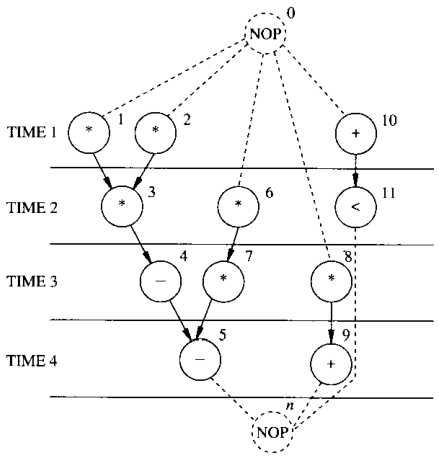
\includegraphics[width=\textwidth]{./Cap5/Images/Image01.png}
        \caption{Scheduled  sequencing  graph}
   		\label{fig:SchSeqG}
    \end{subfigure}
    \quad\quad\quad
    \begin{subfigure}[b]{0.45\textwidth}
        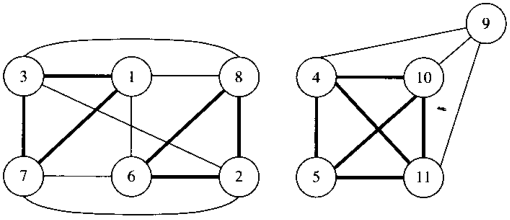
\includegraphics[width=\textwidth]{./Cap5/Images/Image02.png}
        \caption{Compatibility graph of the multiplier and the ALU types}
   		\label{fig:Compat}
    \end{subfigure}
    \caption{}
\end{figure}
An alternative way of looking at the problem is to consider the  conflicts  between operation pairs. Two operations have a conflict when they are not compatible. Conflicts can be represented by  conflict graphs.
\bigskip \\
The \textbf{resource conflict graph} $ G_{-}(V,E) $ is a graph whose vertex set $ V = \lbrace v_i,i=1,2,...,n_{ops} \rbrace $ is in one-to-one correspondence  with  the operations and 	whose edge set $ E = \lbrace \lbrace v_i, v_j \rbrace ,i,j=1,2,...,n_{ops} \rbrace $ denotes  the conflicting operation pairs.
\bigskip \\
A  proper vertex coloring of the conflict graph provides a solution to the sharing problem: each color corresponds to a resource instance. All vertexes connected must have different colors.\\
\textbf{An optimum resource sharing} corresponds to a vertex coloring with a minimum number of colors. Such a number is the  \textit{chromatic number} denoted by $ \chi $.  Note that $ K= \chi $

\paragraph{Example}
Consider again the scheduled sequencing graph of Figure \ref{fig:SchSeqG}. We show in Figure  \ref{fig:ConfGr}  the conflict graphs for the multiplier and  ALU  types. Examples of independent sets are   among others. Each graph  can  he colored with two colors, yielding an overall resource requirement of  4.
\begin{figure}[H]
    \centering
    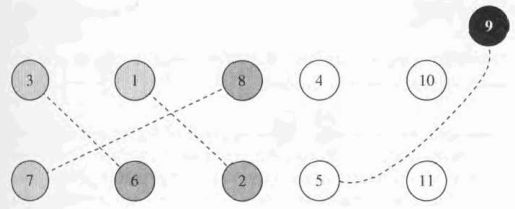
\includegraphics[width=0.45\textwidth]{./Cap5/Images/Image03.png}
    \caption{Conflict  graphs  for  the  multiplier  and  ALU  types}
    \label{fig:ConfGr}
\end{figure}	
Exact and heuristic solution methods have been proposed to solve the \textit{clique partitioning} and \textit{vertex coloring} problems.


\subsection{Resource Sharing}
Two operations are compatible  if  they can be implemented by resources of the same type and if they are not concurrent. Therefore, the \textit{compatibility graph} $ G_{+}(V,E) $ is described by the a set of edges that connect two operations of the same operation type and have different start time. Such a graph can be constructed by traversing the sequencing graph. This graph is a \textit{comparability graph} because it has a transitive orientation property. Indeed, a corresponding directed graph could be derived by assigning an orientation to the edge.
\begin{figure}[H]
    \centering
    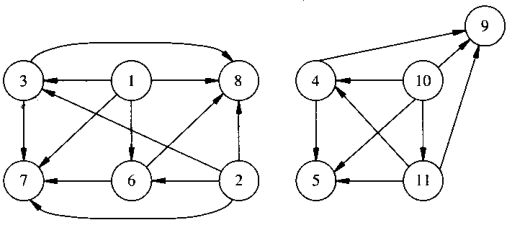
\includegraphics[width=0.45\textwidth]{./Cap5/Images/Image06.png}
    \caption{Transitive  orientation  of  the compatibility  graph for the multiplier and for the ALU types}
    \label{fig:Transi}
\end{figure}

Let us consider now the \textit{conflict graphs} for each resource type. Vertices correspond to  intervals  and  e edges correspond to interval intersection. Hence they are \textit{interval graphs}. The search for a minimum coloring of an interval graph can be achieved in polynomial time.  A  few algorithms can  be  used, including the Golumbic’s algorithm and \textit{LEFT-EDGE}  algorithm.
\begin{figure}[H]
    \centering
    \begin{subfigure}[b]{0.2\textwidth}
        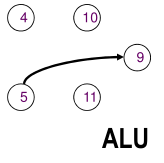
\includegraphics[width=\textwidth]{./Cap5/Images/Image09.png}
        \caption{}
   		\label{fig:mul}
    \end{subfigure}
    \quad\quad\quad
    \begin{subfigure}[b]{0.2\textwidth}
        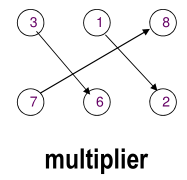
\includegraphics[width=\textwidth]{./Cap5/Images/Image08.png}
        \caption{}
   		\label{fig:alu}
    \end{subfigure}
    \quad\quad\quad
    \begin{subfigure}[b]{0.45\textwidth}
        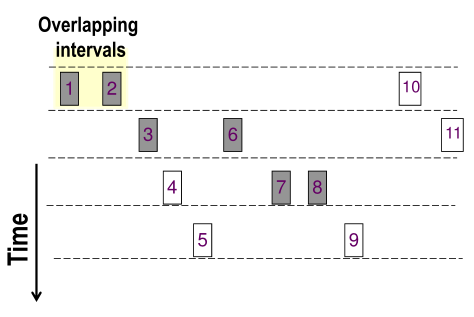
\includegraphics[width=\textwidth]{./Cap5/Images/Image07.png}
        \caption{Overlapping intervals}
   		\label{fig:Overlapping intervals}
    \end{subfigure}
    \caption{}
\end{figure}

\paragraph{Left-Edge Algorithm}
is a coloring algorithm applied on an inteval graph. This algorithm takes as input the set of intervals with \textit{left and right edge} and a set of \textit{colors} (initially one). The principles of the algorithm are the following ones:
\begin{enumerate}
	\item Sort the invervals in a \textit{list} by the \textit{left} edge
	\item Assing non overlapping interval to the forst color according with the \textit{sorted list}.
	\item When epossible intevals are exhausted, increase color and repeat.
\end{enumerate}
\begin{figure}[H]
	\centering$  $
	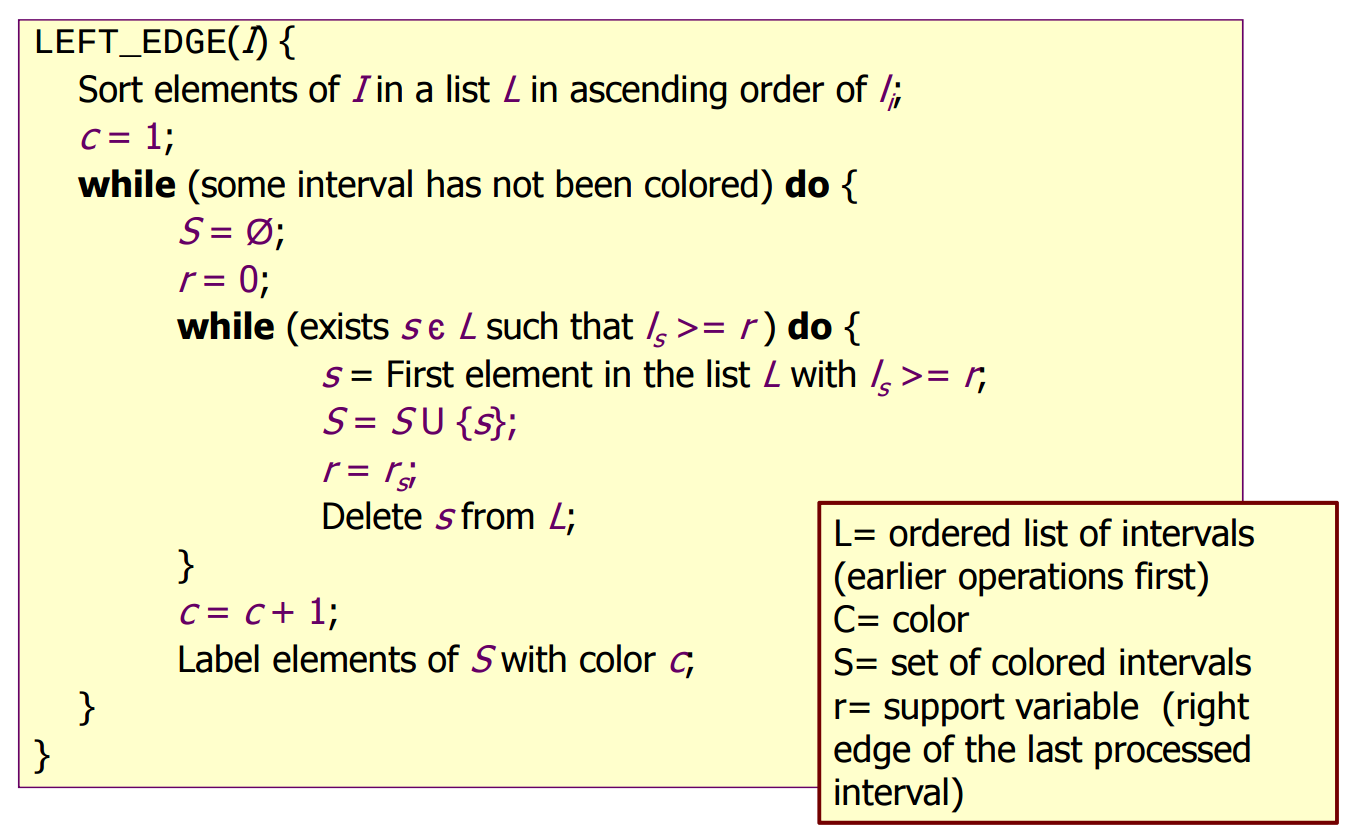
\includegraphics[width=0.60\textwidth]{./Cap5/Images/Image10.png}
	\caption{Pseudo-Code of Left-Edge algorithm}
	\label{fig:PseudoLEalg}
\end{figure}
\begin{figure}[H]
	\centering
	\begin{subfigure}[b]{0.19\textwidth}
		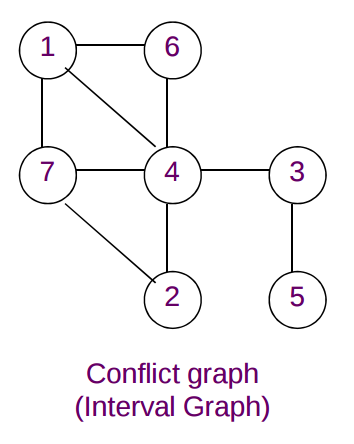
\includegraphics[width=\textwidth]{./Cap5/Images/Image11.png}
		\caption{}
		\label{fig:conflGraph}
	\end{subfigure}
	\quad\quad\quad
	\begin{subfigure}[b]{0.19\textwidth}
		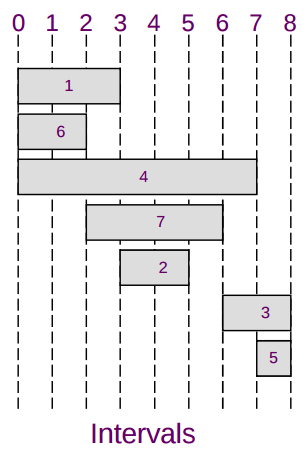
\includegraphics[width=\textwidth]{./Cap5/Images/Image12.png}
		\caption{}
		\label{fig:intervalsLE}
	\end{subfigure}
	\quad\quad\quad
	\begin{subfigure}[b]{0.2\textwidth}
		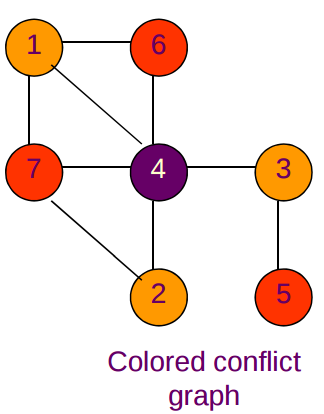
\includegraphics[width=\textwidth]{./Cap5/Images/Image13.png}
		\caption{}
		\label{fig:coloredConflict}
	\end{subfigure}
	\begin{subfigure}[b]{0.2\textwidth}
		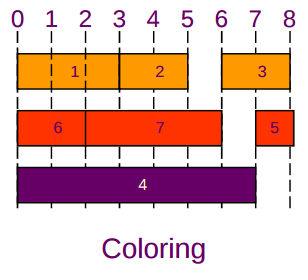
\includegraphics[width=\textwidth]{./Cap5/Images/Image14.png}
		\caption{}
		\label{fig:coloring}
	\end{subfigure}
	\caption{}
\end{figure}
\subsection{Register Sharing}
Registers are used to hold values of variables and to share them we have to consider their \textit{lifetime} (interval between the generation and the last reference of a variable). Variables that are alive in different intervals or under alternative conditions can share the same register. Such variables are called \textit{compatible}
\bigskip\\
Starting from a schedule and assuming that variables with multiple assignment are aliased, we can derive the lifetime of each variables and build a \textit{Conflict Graph} similar to previous ones but this time: 
\begin{enumerate}
	\item Vertices $\longleftrightarrow$ variables.
	\item Edges $\longleftrightarrow$ Overlaps (between variables lifetime)
\end{enumerate}
Next, we can build the \textbf{Compatibility} Graph that complement the conflict graph and show us.
\paragraph{Algorithm: }
Starting from a lifetime conflict graph, our goal is to find the \textit{minimum} number of registers storing all the variables. To reach this goal we can use the \textit{Left-Edge algorithm} (polynomial complexity) but if there are iterative conflict (some variables are alive across the iteration boundary) coloring problem is intractable, so we have to use heuristic algorithms.
\subsection{Bus Sharing and Binding}
Busses act as transfer resources that feed data to functional resources. The operation of writing a specific bus can be modeled explicitly as a vertex in the sequencing graph model. In this case, the compatible (or conflicting) data transfers may be represented by compatibility (or conflict) graphs, as in the case of functional resources.
\bigskip\\
Two problems then arise:
\begin{enumerate}
	\item Find the minimum number of busses to accommodate all (or part of) the data transfers
	\item Find the maximum number of
	data transfers that can be done through a given number of busses.
\end{enumerate}
These problems are analogous to the multi-port binding problem and can be modeled by \textit{ILP constraints}.
\subsection{Module Selection Problem}
The resource-type selection problem, called also module selection, is a \textit{generalization of the binding problem}, where we assume that more than one resource type can match the functional requirements of an operation type. We say that two resource types are \textbf{compatible} if they can perform the same operation. An example is given by the addition operation and the resource types corresponding to \textit{ripple-carry} and \textit{carry look-ahead} adders. Both resource types fulfill the required functionality, but with different area and propagation delay that are the decision variables for this type of problem.
\bigskip\\
Several \textit{heuristic methods} have been proposed for the module selection problem. When a minimum-latency schedule is the goal, the fastest resource types are used in scheduling. Resource sharing and module selection are then applied to minimize the area, in that case slower and smaller resources can be assigned to non-critical operations.

\paragraph{Data path synthesis}
is applied after resource binding and produce: the connection of resources to \textit{multiplexers busses and registers}, interface towards control unit and \textit{I/O ports}.

\begin{figure}[H]
	\centering
	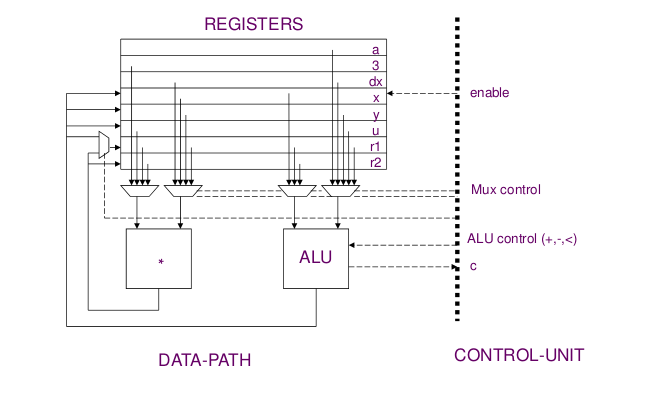
\includegraphics[width=0.50\textwidth]{./Cap5/Images/Image15.png}
	\caption{Example of Data path synthesis}
	\label{fig:dpsynth}
\end{figure}

\paragraph{Control synthesis}
is referred to the synthesis of the control unit starting from scheduling model and obtaining a \textit{syncronous FSM}. The phisical implementation of the control unit can be done with \textit{Hard wired FSM} 
\begin{itemize}
	\item \textit{Hard wired} FSM 
	\item Memory-based Microcode (programmable)
\end{itemize} 

\begin{figure}[H]
	\centering
	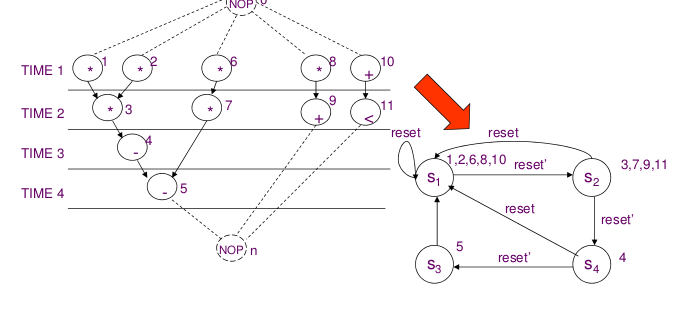
\includegraphics[width=0.60\textwidth]{./Cap5/Images/Image16.png}
	\caption{Example of Control synthesis}
	\label{fig:contrsynth}
\end{figure}

\begin{figure}[H]
	\centering
	\begin{subfigure}[b]{0.30\textwidth}
		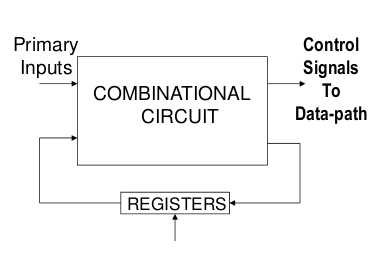
\includegraphics[width=\textwidth]{./Cap5/Images/Image17.png}
		\caption{}
		\label{fig:hardWiredCU}
	\end{subfigure}
	\quad\quad\quad
	\begin{subfigure}[b]{0.30\textwidth}
		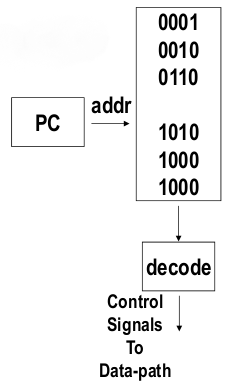
\includegraphics[width=\textwidth]{./Cap5/Images/Image18.png}
		\caption{}
		\label{fig:programCU}
	\end{subfigure}
	\caption{Possible Implementation of Control Unit}
\end{figure}
